\documentclass[12pt,a4paper]{article}
\usepackage[utf8]{inputenc}
\usepackage[polish]{babel}
\usepackage[T1]{fontenc}
\usepackage{geometry}
\usepackage{graphicx}
\usepackage{hyperref}
\usepackage{listings}
\usepackage{xcolor}
\usepackage{pdfpages}

\geometry{margin=2.5cm}

% Konfiguracja wyświetlania kodu w LaTeX
\lstset{
    language=C++,
    basicstyle=\ttfamily\small,
    keywordstyle=\color{blue}\bfseries,
    stringstyle=\color{red},
    commentstyle=\color{green!60!black},
    numbers=left,
    numberstyle=\tiny\color{gray},
    stepnumber=1,
    breaklines=true,
    frame=single,
    tabsize=4,
    showstringspaces=false
}

\title{\textbf{Sprawozdanie z Projektu: Lista Dwukierunkowa na Stercie z Wykorzystaniem Wzorców Projektowych oraz Narzędzi Doxygen i Git}}
\author{\textbf{Krzysztof Zdzieszyński} \\ Akademia Nauk Stosowanych w Nowym Sączu}
\date{\today}

\begin{document}

\maketitle
\tableofcontents
\newpage

\section{Rozdział 1: Ogólne określenie wymagań}

Celem niniejszego projektu było opracowanie i przetestowanie modułowej implementacji dwukierunkowej listy wiązanej działającej na stercie w języku C++, z uwzględnieniem dobrych praktyk inżynierii oprogramowania oraz nowoczesnych narzędzi deweloperskich.

\subsection{Wymagania funkcjonalne i programistyczne}
\begin{itemize}
    \item \textbf{Modułowość kodu:} Podział struktury na osobne pliki nagłówkowe (\texttt{Node.h}, \texttt{Iterator.h}, \texttt{DoublyLinkedList.h}, \texttt{ListFactory.h}).
    \item \textbf{Wzorce projektowe:} Zastosowanie wzorca \textit{Factory} (Fabryka) do bezpiecznego tworzenia obiektów listy na stercie oraz wzorca \textit{Iterator} do sekwencyjnej nawigacji po węzłach.
    \item \textbf{Operacje na liście:}
    \begin{itemize}
        \item Dodawanie elementu na początek, na koniec oraz pod wskazany indeks.
        \item Usuwanie elementu z początku, z końca oraz spod wskazanego indeksu.
        \item Wyświetlanie całej listy od początku oraz w odwrotnej kolejności.
        \item Swobodne przechodzenie do następnego oraz poprzedniego elementu przy użyciu iteratora.
        \item Czyszczenie całej listy i poprawne zwalnianie pamięci sterty.
    \end{itemize}
\end{itemize}

\subsection{Wymagania dotyczące narzędzi i dokumentacji}
\begin{itemize}
    \item \textbf{Doxygen:} Automatyczne wyciąganie komentarzy z kodu źródłowego i wygenerowanie dokumentacji technicznej w formacie \LaTeX{} kompilowanej do pliku \texttt{refman.pdf}.
    \item \textbf{System kontroli wersji Git:} Rejestracja historii zmian w serwisie GitHub obejmująca:
    \begin{itemize}
        \item Wykonanie co najmniej 5 commitów.
        \item Przetestowanie cofnięcia się o dwa commity.
        \item Usunięcie wskazanego commita z historii.
        \item Synchronizację pracy między dwiema różnymi lokalizacjami na komputerze.
        \item Symulację usunięcia pliku z projektu, wywołanie błędu kompilacji i przywrócenie poprawnej wersji z repozytorium GitHub.
    \end{itemize}
\end{itemize}
\newpage

\section{Rozdział 2: Analiza problemu}

\subsection{Struktura danych listy dwukierunkowej}
Lista dwukierunkowa to liniowa struktura danych składająca się z węzłów alokowanych dynamicznie na stercie. Każdy węzeł zawiera wartość przechowaną oraz dwa wskaźniki: na następny (\texttt{next}) i poprzedni (\texttt{prev}) element. Taka architektura pozwala na wykonywanie operacji na obu krańcach ze złożonością czasową $O(1)$.

\subsection{Wzorce projektowe}
\begin{enumerate}
    \item \textbf{Wzorzec Factory (Fabryka):} Klasa \texttt{ListFactory} umożliwia enkapsulację procesu tworzenia listy na stercie (\texttt{new DoublyLinkedList<T>()}). Chroni to kod kliencki przed bezpośrednim zarządzeniem pamięcią przy tworzeniu instancji.
    \item \textbf{Wzorzec Iterator:} Klasa \texttt{ListIterator} abstrahuje proces przechodzenia po strukturze danych. Pozwala to na dostęp do elementów bez konieczności ujawniania wewnętrznych połączeń wskaźnikowych.
\end{enumerate}

\subsection{Systemy wspierające: Git oraz Doxygen}
System \textbf{Git} umożliwia pracę wieloetapową, śledzenie zmian w plikach oraz odzyskiwanie spójnego stanu aplikacji po uszkodzeniach. \textbf{Doxygen} natomiast analizuje specjalne bloki komentarzy w kodzie źródłowym i generuje pełny wykaz klas, metod oraz pól w formacie \LaTeX{}, z którego tworzony jest plik PDF.
\newpage

\section{Rozdział 3: Projektowanie}

Projekt został zaprojektowany z zachowaniem zasady pojedynczej odpowiedzialności (SRP), gdzie każda klasa znajduje się w osobnym pliku nagłówkowym:

\begin{itemize}
    \item \texttt{Node.h} -- generyczna struktura pojedynczego węzła przechowywana na stercie.
    \item \texttt{Iterator.h} -- klasa \texttt{ListIterator} realizująca przeglądanie elementów w przód i w tył.
    \item \texttt{DoublyLinkedList.h} -- główna klasa zarządzająca węzłami na stercie, realizująca operacje wstawiania, usuwania i wyświetlania.
    \item \texttt{ListFactory.h} -- klasa fabryki odpowiedzialna za alokację listy.
    \item \texttt{main.cpp} / \texttt{test\_lista\_dwukierunkowa.cpp} -- moduły testowe sprawdzające poprawne działanie wszystkich metod.
\end{itemize}
\newpage

\section{Rozdział 4: Implementacja}

\subsection{Kluczowe metody klasy DoublyLinkedList}
Poniżej przedstawiono implementację metody dodawania elementu pod wskazany indeks z zachowaniem poprawności wskaźników \texttt{next} oraz \texttt{prev}:

\begin{lstlisting}[caption={Dodawanie elementu pod podany indeks}]
void addAt(int index, const T& val) {
    if (index < 0 || index > count) {
        throw std::out_of_range("Indeks poza zakresem!");
    }
    if (index == 0) {
        addFront(val);
    } else if (index == count) {
        addBack(val);
    } else {
        Node<T>* current = getNodeAt(index);
        Node<T>* newNode = new Node<T>(val);
        Node<T>* prevNode = current->prev;

        prevNode->next = newNode;
        newNode->prev = prevNode;
        newNode->next = current;
        current->prev = newNode;
        count++;
    }
}
\end{lstlisting}

\subsection{Repozytorium Git oraz historia commitów}
\begin{itemize}
    \item \textbf{Adres repozytorium GitHub:} \url{https://github.com/KrzysztofZdzieszynski/lista-dwukierunkowa}
\end{itemize}

W ramach pracy z systemem kontroli wersji rejestrowano postępy w repozytorium. Poniżej przedstawiono pełny log z historii commitów (\texttt{git log --oneline --graph --all}):

\begin{lstlisting}[caption={Rzeczywista historia commitów z systemu Git}]
* da16ced (HEAD -> main, origin/main) Commit 5: Dodanie wzorca Factory, wyswietlania wstecz oraz pliku main.cpp
* 2b3b477 Commit 4: Implementacja wzorca Iteratora oraz integracja z klasa listy
* 43acabd Commit 3: Dodanie metod removeFront, removeBack oraz czyszczenia listy
* 181c786 Commit 2: Dodanie metod addFront, addBack oraz wyswietlania listy
* e3a06e8 Commit 1: Dodanie struktury Node i bazowego szkieletu klasy listy
\end{lstlisting}

\subsection{Weryfikacja scenariuszy w Git}
\begin{enumerate}
    \item Utworzono 5 chronologicznych commitów dokumentujących postęp prac.
    \item Przeprowadzono testowy powrót w historii o dwa commity wstecz za pomocą polecenia \texttt{git reset --hard HEAD}.
    \item Sklonowano repozytorium do drugiego katalogu na dysku, wprowadzono zmiany, wysłano je na serwer zdalny (\texttt{git push}) i zsynchronizowano w pierwotnej lokalizacji przy użyciu \texttt{git pull}.
    \item Celowo usunięto plik \texttt{ListFactory.h}, wywołując błąd kompilacji, a następnie przywrócono go poleceniem \texttt{git checkout ListFactory.h}.
\end{enumerate}

\subsection{Generowanie dokumentacji Doxygen}
Plik konfiguracyjny \texttt{Doxyfile} został wygenerowany poleceniem \texttt{doxygen -g Doxyfile} z włączoną opcją \texttt{GENERATE\_LATEX = YES}. Wynikowe pliki trafiły do katalogu \texttt{latex/}, po czym zostały skompilowane poleceniem \texttt{pdflatex refman.tex} do pliku \texttt{refman.pdf}.
\newpage

\section{Rozdział 5: Wnioski końcowe}

W wyniku realizacji projektu powstała w pełni funkcjonalna implementacja dwukierunkowej listy wiązanej na stercie w języku C++. Zastosowanie wzorców projektowych \textit{Factory} i \textit{Iterator} zwiększyło czytelność oraz elastyczność kodu.

Integracja generatora \textbf{Doxygen} z systemem \textbf{\LaTeX{}} pozwoliła na sprawną automatyzację powstawania dokumentacji technicznej API. Ćwiczenia praktyczne z narzędziem \textbf{Git} pozwoliły na opanowanie kluczowych mechanizmów kontroli wersji, wycofywania błędnych zmian oraz pracy z repozytorium zdalnym GitHub.

\newpage
\appendix
\section{Załącznik: Dokumentacja techniczna Doxygen}
Poniżej dołączono dokumentację techniczną wygenerowaną automatycznie przez program Doxygen do pliku PDF.

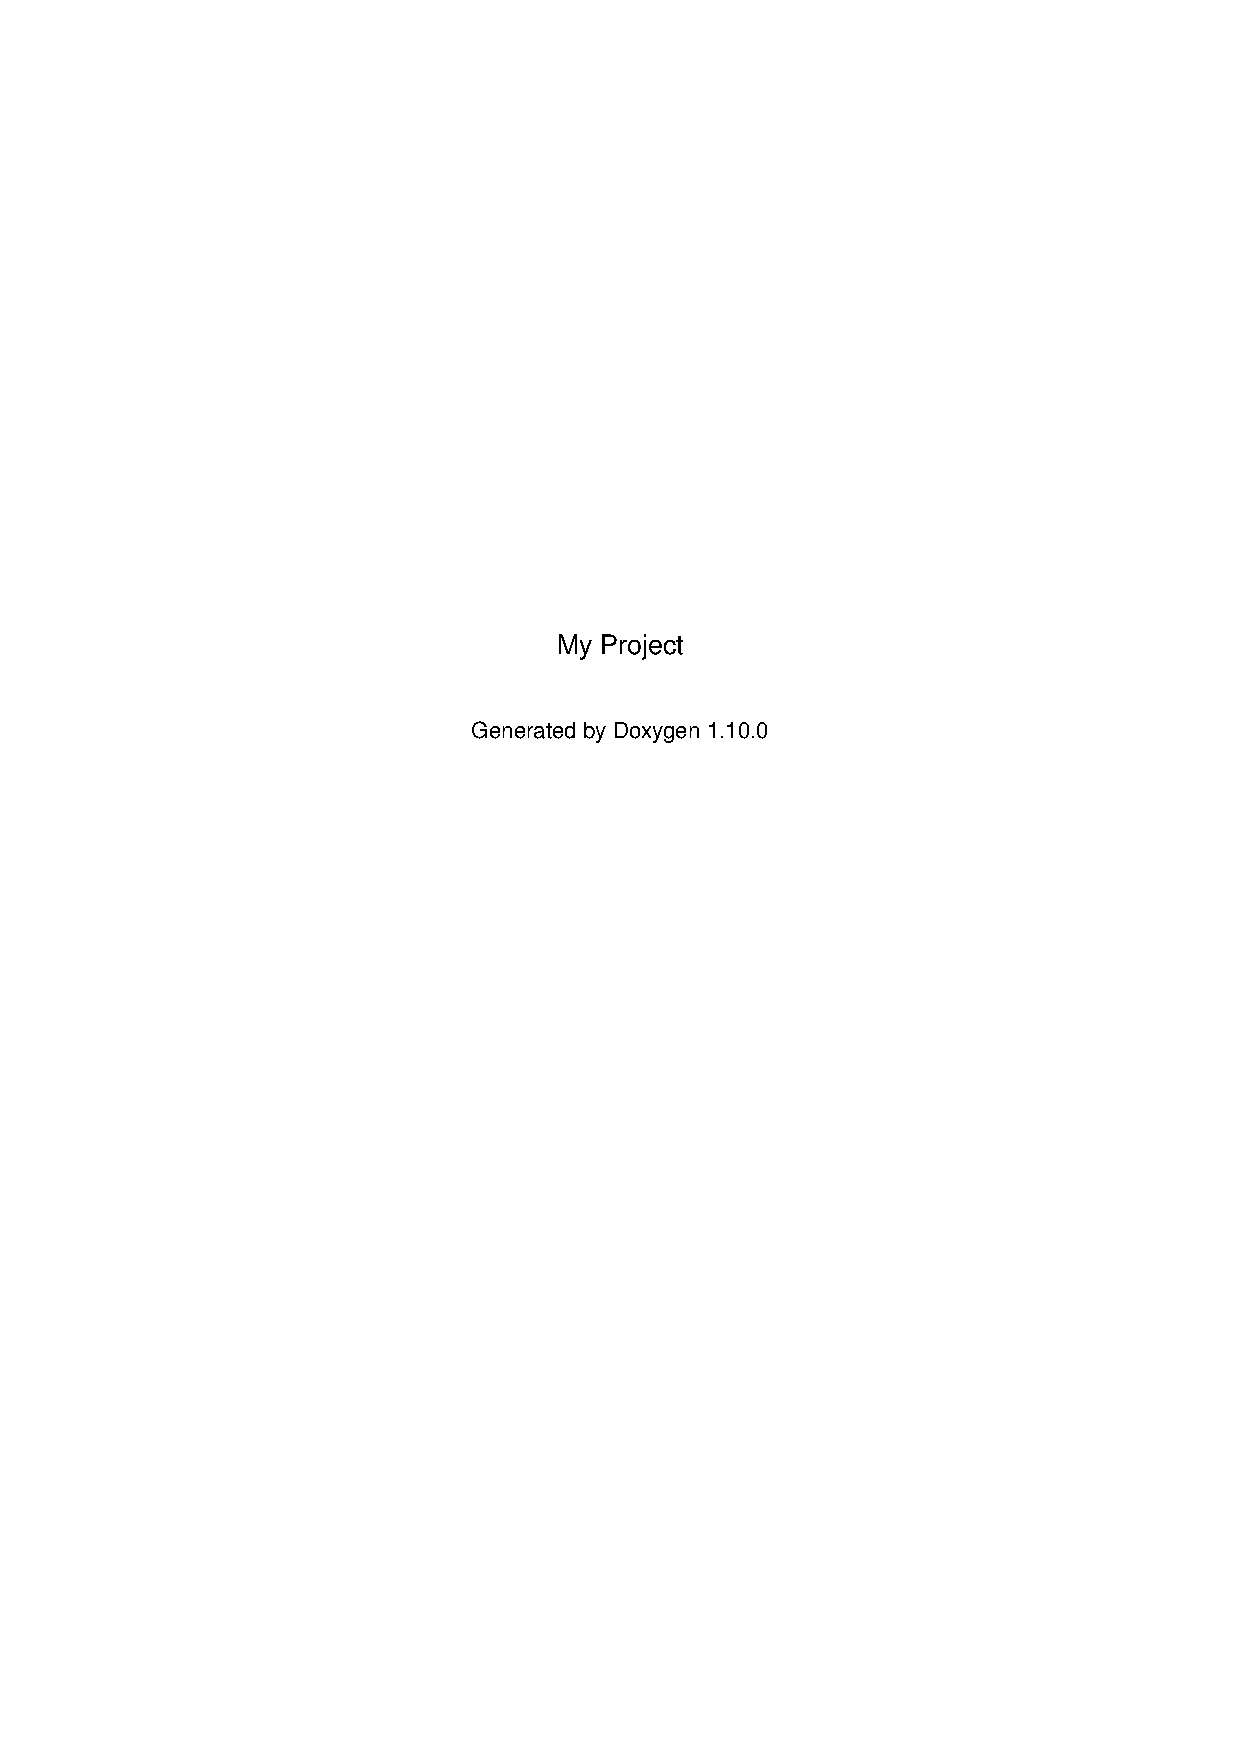
\includepdf[pages=-]{latex/refman.pdf}

\end{document}